% !TEX program = xelatex
\documentclass[12pt]{ctexart}
\usepackage{multirow,graphicx,textcomp,bigstrut,float,syntonly,amsmath,amsfonts,amssymb,etoolbox,indentfirst,bm,subfigure}
\usepackage{amsmath}
\usepackage{amssymb}
\usepackage{algorithm}
\usepackage{algorithmicx}
\usepackage{algpseudocode}
\CTEXoptions[today=old]
\CTEXsetup[format={\Large\bfseries}]{section}
\title{Report}
\author{Li Hanyu}
\date{\today}
\begin{document}
\maketitle
\newpage
\section{Labels}
\par Every combination of SPE and IFE will be transformed into a 12-dimension 0-1 vector like [1, 0, 1, 0, 0, 0, 0, 1, 0, 0, 0, 1]. Above is the label of lgG $\lambda$ situation.

\begin{tabular}{|c|c|c|c|c|c|c|}
    \hline
    component&1&2&3&4&5&6\\
    \hline
    related columns&lgG,$\kappa$&lgG,$\lambda$&lgA,$\kappa$&lgA,$\lambda$&lgM,$\kappa$&lgM,$\lambda$\\
    \hline
    wheather 0 or 1&\multicolumn{6}{|c|}{1 if obvious peaks have same position}\\
    \hline
    \hline
    component&0&7&8&9&10&11\\
    \hline
    related columns&overall&lgG&lgA&lgM&$\kappa$&$\lambda$\\
    \hline
    wheather 0 or 1&only 0 when 7-11 is 0&\multicolumn{5}{|c|}{1 if obvious peaks are detected}\\
    \hline
    \end{tabular}
\begin{enumerate}
    \item The first component is the overall judgement(1 if abnormal and 0 if normal).
    \item The next 6 components are the links between heavy chain(lgG, lgA, lgM) and light chain($\kappa$ and $\lambda$). For example, if lgG and $\lambda$ has the same peak position, then the third component will be 1, because the order is:G$\kappa$, G$\lambda$, A$\kappa$, A$\lambda$, M$\kappa$, M$\lambda$.
    \item The last 5 components are wheather hard and strong edges(obvious peak) are detected in the corresponding column of IFE.
\end{enumerate}
\section{Classification Rules}
\par After reading in a picture of SPE and IFE like:(lgG and $\lambda$ situation)
\begin{figure}[H]
    \centering
    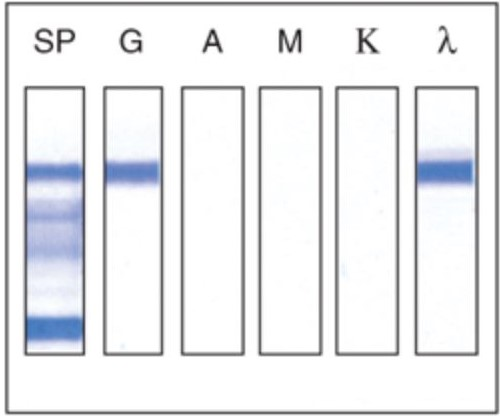
\includegraphics[width=0.5\linewidth]{gl.jpg}
\end{figure}
cv2.fastNlMeansDenoising are applied to every column of the electrophoresis result. Six density plots are then analysed according to the columns.
\begin{figure}[H]
    \centering
    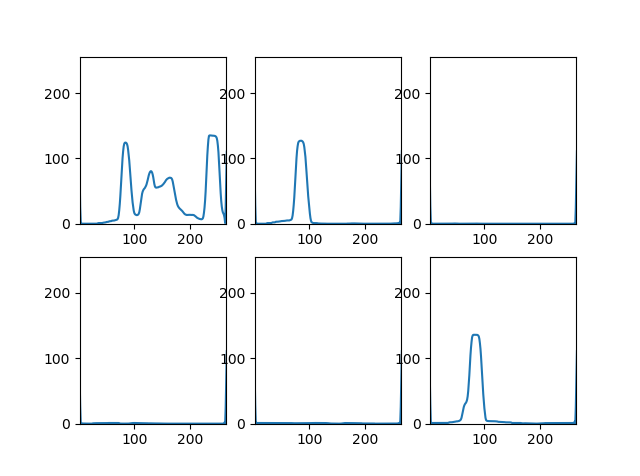
\includegraphics[width=0.5\linewidth]{lgG-lambda.png}
\end{figure}
Afterwards, we apply cv2.Sobel(take derivative) to the density plots and find the max, max position, min, min position of the derivative curve. The column will be labelled as abnormal in the last five components of the label if the $\frac{max(f')+|min(f')|}{2}$ is higher than a formerly set threshold $t_1$. The link between certain kinds of heavy and light chain will be noticed if the difference of the peak position (which is determined by the mean of max position and min position) of the two chains are less than another threshold $t_2$, and both $\frac{max(f')+|min(f')|}{2}$ are higher than threshold $t_3$.
\section{Instances}
For normal and polyclonal increase instances:
\subsection{normal}
\begin{figure}[H]
    \centering
    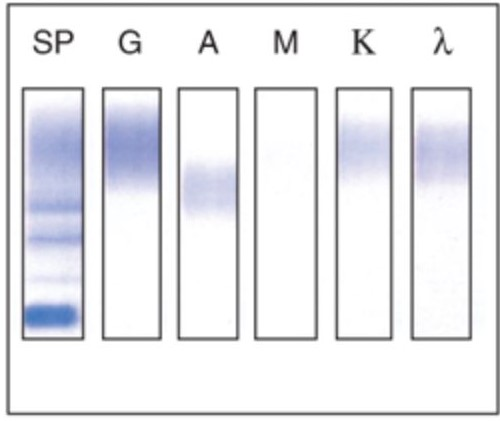
\includegraphics[width=0.5\linewidth]{no.jpg}
\end{figure}
\begin{figure}[H]
    \centering
    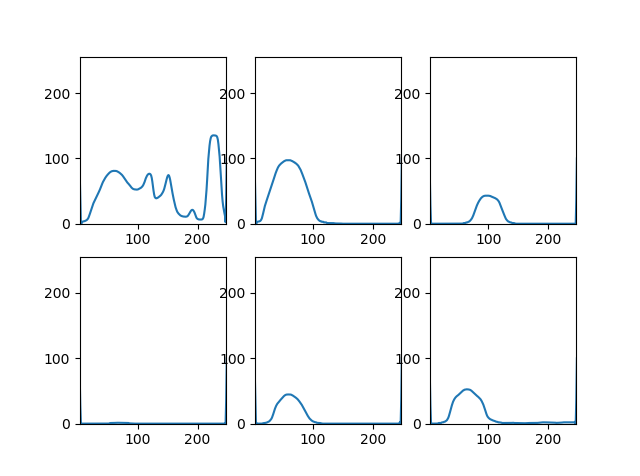
\includegraphics[width=0.5\linewidth]{normal.png}
\end{figure}
label: [0, 1, 1, 0, 0, 0, 0, 0, 0, 0, 0, 0]
\subsection{polyclonal increase}
\begin{figure}[H]
    \centering
    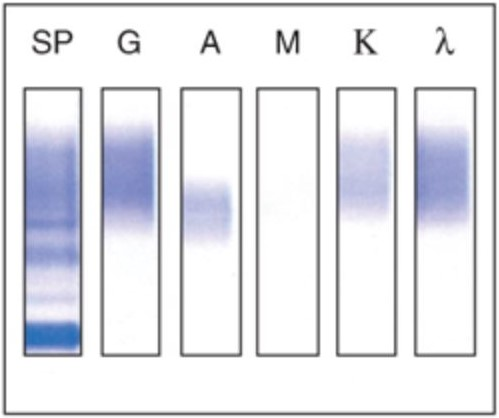
\includegraphics[width=0.5\linewidth]{pr.jpg}
\end{figure}
\begin{figure}[H]
    \centering
    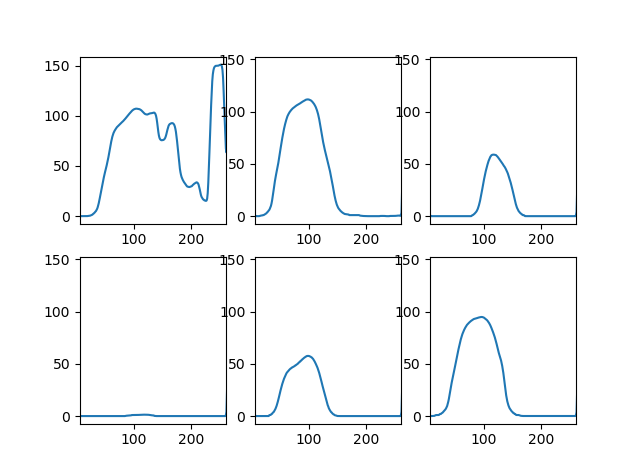
\includegraphics[width=0.5\linewidth]{polyclonal-increase.png}
\end{figure}
label:[0, 1, 1, 0, 0, 0, 0, 0, 0, 0, 0, 0]
\end{document}